\documentclass[a4paper, 12pt]{article}
\usepackage[utf8]{inputenc}
\usepackage[francais]{babel}
%\usepackage[T1]{fontenc}
\usepackage{graphicx}
\usepackage{hyperref}
\usepackage{epstopdf}
\usepackage[table]{xcolor}
\usepackage{caption}
\usepackage{colortbl,hhline}
\title{Informatique et Science Du Numérique}
\date{\today}
\author{Gnebehi Bagre Jean Philippe ET Sow Mamadou Binta}

\begin{document}
	\maketitle
	
\newpage
	\tableofcontents
	
\newpage

\begin{minipage}{.9\textwidth}%
	\listoffigures \addcontentsline{toc}{section}{Table des figures} 
	\vspace{5cm}
	\listoftables \addcontentsline{toc}{section}{Liste des tables} 
\end{minipage}

\newpage

\vspace*{\stretch{1}}
	\begin{abstract}

Les cours \cite{ISN1} d'\textcolor{blue}{ISN}\footnote{Informatique des sciences du Numérique}  se dérouleront par le biais de différentes activités comme des débats, des exposés, des travaux pratiques et des projets. Les activités sont organisées autour d'une équipe d'élèves. Elles permettent de mettre en œuvre les savoirs et capacités acquis au cours de l'année.
	\end{abstract}
\vspace*{\stretch{1}}

	\newpage
\begin{center}
	\section{Les activités}
\end{center}
      
   Les activités principalement développées lors des cours d'ISN sont « les projets ». Ces projets sont réalisés par les élèves sous la conduite du professeur. Ils permettent de pouvoir traiter certaines parties du programme en toute autonomie, mais ils peuvent aussi porter sur des problématiques issues d'autres disciplines.
Le développement d'un projet permet d'acquérir les compétences suivantes:

      \begin{itemize}

\item Proposer une approche qui réponde au cahier des charges
\item Mener des recherches documentaires
\item Gérer les étapes de l'avancement d'un projet
\item Concevoir un projet en autonomie

      \end{itemize}

          \subsection{Des exemples de projets}
 \begin{center}
 \end{center}         
 \captionof{table}{Exemple de projet d'ISN}
    \begin{tabular}{|l|l|l|} \hline    

\textbf{Nom du projet} & \textbf{Site Web} & \textbf{Lycée}\\ \hline
    
Cubesta&\href{http://cubesta-project.github.io/CubeSTA/}{cubesta-project.github.io}&Lycée du Forez (Feurs - Loire)\\ \hline 
    
Crazy Game&\href{http://www.yorka-design.fr/ISN/}{www.yorka-design.fr}&Lycée Arthur Varoquaux Tomblaine \\ \hline

    \end{tabular}
    
      \section{Éléments du programme}
Ce cours est enseigné deux heures par semaine. Le programme est composé de quatre parties: \textbf{ Représentation de l’information, algorithmique, langage et programmation, architectures matérielles etc...}
\vfill
\begin{center} 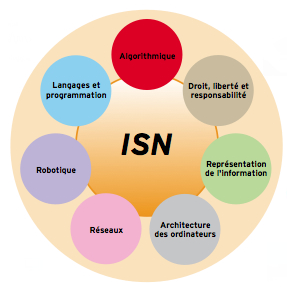
\includegraphics[scale=0.6]{isn.png} \end{center}
\vfill

      \subsection{Représentation de l'information}
  
  \subsubsection{La représention binaire}
  	Le système binaire est un système de numération utilisant la base 2. On nomme couramment bit (de l'anglais binary digit, soit « chiffre binaire ») les chiffres de la numération binaire positionnelle. Ceux-ci ne peuvent prendre que deux valeurs, notées par convention 0 et 1.

C'est un concept essentiel de l'informatique. En effet, les processeurs des ordinateurs actuels sont composés de transistors ne gérant chacun que deux états.
\vfill
\begin{flushright} 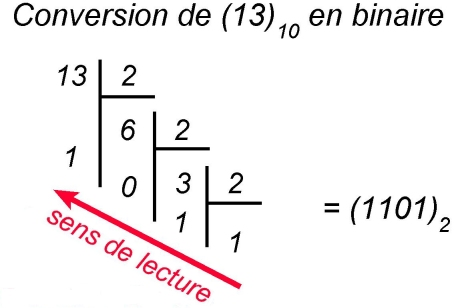
\includegraphics[scale=0.5]{isn2.jpg} \end{flushright}
\vfill
  	
  	\subsubsection{Numérisation}
  L'ordinateur \cite{ISN2} manipule uniquement des valeurs numériques. Une étape de numérisation des objets du monde physique est donc indispensable.
  \begin{figure}[!h]
  \centering
  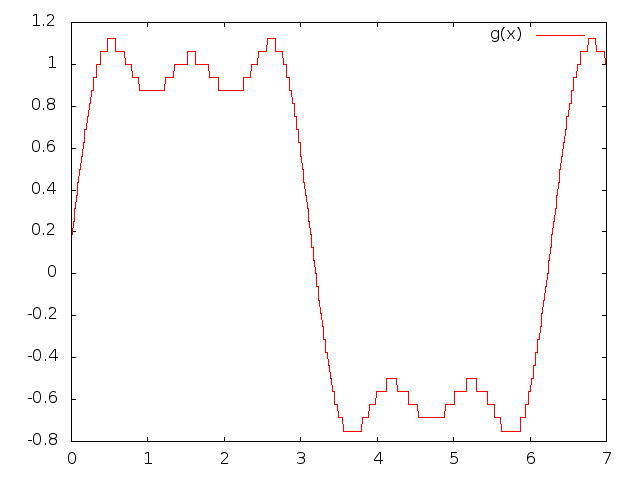
\includegraphics[scale=0.3]{graphe1.png}
  \caption{Exemple Signal de Numérisation}
  \end{figure}
  
\subsection{\textbf{Algorihtmique}}
\subsubsection{\textit{Algorithmique simple}}
\begin{itemize}
\item [*]Rechercher un élément dans un tableau trié par une méthode dichotomique:
La recherche dichotomique est une manière efficace et rapide de rechercher un élément dans une structure de données triée. \href{http://openclassrooms.com/courses/recherche-dichotomique}{Voir le lien ici}
\item [*]Trier un tableau par sélection:
	L'idée est simple : rechercher le plus grand élément (ou le plus petit), le placer en fin de tableau (ou en début) et assurer la suite du tri. \href{http://openclassrooms.com/courses/le-tri-par-selection}{Plus de détail}
\end{itemize}

\subsubsection{\textit{Algorithmique Avances}}
    \begin{itemize}
    \item [$\bullet$] Tri par fusion:
    Le principe de cet algorithme est très simple. Il consiste à fusionner deux sous-séquences triées en une séquence triée.\\
     
   \begin{figure}[!h]
  \centering
    \begin{center}
	38		27		43		3\\

$\swarrow$  $\searrow$\\
	38		27	\hspace{1cm}	43		3\\
$\swarrow$\hspace{2cm}$\searrow$\\
38\hspace{0.5cm}27\hspace{2.5cm}43\hspace{0.5cm}3\\
$\searrow$\hspace{2.5cm}$\swarrow$\\
27		38 \hspace{1cm}	3 	43\\
$\searrow$\hspace{1cm}$\swarrow$\\
$\searrow$\hspace{0.1cm}$\swarrow$\\
3	27	38		43\\
	  \end{center}
	  \caption{\textcolor{brown}{Exemple de tri par fusion}}
  \end{figure}
    \end{itemize}
\subsection{\textbf{Langage et Programmation}}
\subsubsection{\textit{Fonction}} 
En ISN, une fonction est une routine qui retourne une valeur.\\
Une fonction possède:\\
$\bullet$ Un nom\\
$\bullet$ Des paramètres comportant chacun un nom et un type\\
$\bullet$ Un type de sa valeur de retour\\
$\bullet$ Un bloc de code qui est celui de la fonction\\
$\bullet$ L'affectation d'un résultat à une variable qui est sa valeur de retour.

\subsubsection{\textit{Langages de description}}
\begin{center}
 \end{center}         
\begin{table}[!h]
\rowcolors{1}{lightgray}{gray}
\begin{tabular}{|l||p{12cm}|} \hline
Savoir & Présentation du langage HTML\cite{ISN3}. et du principe de séparation du contenu et de la mise en forme.\\ \hline \hline
Capacités & Créer et analyser une page web en langage HTML.\\ \hline \hline
Observation & On met en valeur le double usage du langage, lisible par un humain et interprétable par une machine. On utilise HTML pour écrire une page « à la main », puis on insiste sur le fait que ce langage sert aussi de cible à des générateurs de pages. On évalue la qualité des pages du point de vue de la correction syntaxique et de l'efficacité du message.\\ \hline
\end{tabular}
\captionof{table}{Récapitulatif}
\end{table}
\subsection{\textbf{Architectures Materielle}}
\subsubsection{\textit{Architecture des ordinateurs}}
$\bullet$  Éléments d’architecture\\
\href{http://web.isen-bretagne.fr/livres/python/ressources/WEB/00-Chapitres/Chap1-Architecture.pdf}{voir le lien}\\
$\bullet$  Jeu d’instruction\\
Le jeu d'instructions précise non seulement les registres et instructions supportées par le processeur, mais aussi la façon dont ces instructions et les opérandes sont représentés en mémoire.
Chaque instruction machine contient un code qui indique l'instruction à exécuter : addition, multiplication, branchement, etc. Ce code est appelé le code-opération, en abrégé opcode. 
\begin{center}
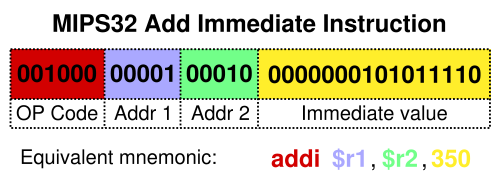
\includegraphics[scale=0.3]{MIPS32_instruction.png}
\end{center}
\subsection{\textbf{Reseau}}

\subsubsection{Transmission point par point}
Le lien ci dessous vous permettra de mieux comprendre:\\
\href{http://www.youtube.com/watch?v=NCpIVzG-ejc}{\textcolor{blue}{TPP}}\footnote{Transmission point par point}
\subsubsection{Adressage sur un réseau}
Cour vidéo de sous-réseaux et de masque de sous réseaux.\\
\href{http://www.youtube.com/watch?v=zlzh1QcBb54}{$\bullet$Ici}
\begin{center}

\vfill
\section{Conclusion}
\end{center}
                La Spécialité ISN \cite{ISN4}. (Informatique et Sciences du Numériques) permet aux élèves des classes de Terminale S (robotique, réseaux internet \cite{ISN5}, algorithmique, programmation en langage objet...), et cela pendant deux heures hebdomadaire.
Les élèves peuvent présenter cette spécialité au baccalauréat. Ils leur faudra pour cela mener un travail de projet en équipe (2 à 5 élèves par équipe) et le présenter à l’oral le jour de l’épreuve (le tout accompagné par un dossier numérique).
Les projets sont variés, laissés à l’initiative des élèves, mais toutefois tempérés par le professeur encadrant la discipline.
\vfill

\newpage

\bibliographystyle{plain}
\bibliography{Bibliography}	

\end{document}
	